\documentclass{article}

\usepackage{listings}
\usepackage{color,soul}
\usepackage{indentfirst}
\usepackage{graphicx}
\usepackage{hyperref}
\usepackage[margin=1.25in]{geometry}

\lstset{
basicstyle=\ttfamily,
columns=flexible,
breaklines=true
}

\title{Areal Unit Segregation in Alabama's 2020 Congressional Districts }
\author{Rebecca Wagner}
\date{}
 
\begin{document}
\maketitle

\begin{abstract}
Monte Carlo simulations have proved useful in redistricting legislation, where the simulation generates districting maps that are used to aproximate the state space of all possible plans. Two such algorithms, Markov Chain Monte Carlo (MCMC) and Sequential Monte Carlo (SMC), begin with a "seed" districting plan and iteratively generate new possible plans according to a set of provided criteria. This paper utilizes data generated with both MCMC and SMC algorithms to examine Alabama's 2020 congressional districting map, which was challenged for racial segregation. We employ Saporito and Maliniak's \hl{(year)} areal unit segregation measure ($S^{+/-}$) to quantitatively measure segregation in the orginial 2020 districting plan and our own algorithmically generated plans. We find that \hl{finish}
\end{abstract}

\section{Introduction}
\subsection{Monte Carlo Simulations in Redistricting}
\par 
In the United States, congressional districts are created for the purpose of electing members to the House of Representatives. In this process, each state is apportioned a number of seats in the House based on it's population. The state is then divided into as many congressional districts as they are granted seats, where one representative may be elected from each district. Every 10 years, states redraw their congressional districts in a process called redistricting, which is intended to ensure that these districts remain a representative sample of voters as populations grow and change over time. However, districts may also be drawn in such a way that they are not representative of the state's population. When this is done purposfully (often in an effort to minimize the voting strength of certain demographic groups) a district is considered to be gerrymandered.
\par
Commonly, gerrmandering occurs when a demographic community is "packed" into a small number of districts so it's voting power is concentrated in these districts, or "cracked" between many districts so it's voting power is diluted across all districts. However, social scientists also know that demographic groups often cluster together naturally, forming natural pockets of high and low populations in a state \hl{cite}. This tendancy makes it difficult to tell whether a district has been gerrymandered based on look or population alone, and leads us to ask how we can systematically tell if a district has been gerrymandered. 
\par
One approach to answering this question relies on the use of Monte Carlo simulations, where districting maps are stochastically generated for analysis. \hl{These generated maps are used to approximate the sample space of redistricting plans in a given state, which can then be quantitatively analyzed to argue whether the enacted plan has been gerrymandered.} However, the issue of generating such a sample space is complex. The Metric Geometry and Gerrymandering Group (MGGG) of Tufts University proposed a Markov Chain Monte Carlo (MCMC) based algorithm to generate sample plans, where the algorithm takes a random walk across the sample space of districing plans. Key to this MCMC algorithm is its lack of memory—each step depends only on the last. Therefore each transformation generates a new map, and a representative space can be generated very quickly \hl{cite}. 
\par
Also key to the MCMC algorithm is exactly how it traverses from one map to the next. MGGG has recently proposed \emph{Recombination} (ReCom) for this process, where the algorithm combines the entirety of two districts and subsequently randomly splits them, creating an entirely new map. On the other hand, the \emph{Flip} proposal relies on flipping nodes of a spanning tree—in essence swapping the district that a single locality belongs to.
MGGG argues that this Flip Proposal does not efficiently explore the space of all possible districting plans, as it has a tendency to draw non-compact plans unless tight constraints are imposed that significantly slow the process. Therefore, while ReCom may be computationally more expensive, it generates much more compact plans in fewer steps than Flip \hl{(DeFord et al, 2021)}. MGGG has made their MCMC with ReCom algorithm publicly available in the Python library \lstinline{GerryChain}. 
\par
Similarly, the Algorithm-Assisted Redistricting Methodology group (ALARM) at Harvard University published \lstinline{Redist}, an open-sourced R package with comparable computational capabilities to \lstinline{GerryChain}. However, instead of Markov Chains, \lstinline{Redist} employs Sequential Monte Carlo (SMC) simulations. While MCMC strategies make small, sequential changes to one “seed” plan, SMC creates many different plans from scratch. The technique draws a random spanning tree on the given state, and selects an edge at random to split and create two sub trees. This step is repeated several times until the appropriate number of districts are created. ALARM states that this SMC strategy is more easily scalable to the kinds of large datasets required for state redistricting, and that it is more efficient \hl{(McCarten and Imani, 2020)}. In any sense, both GerryChain and Redist face limitations in that it is impossible to generate the complete state space of districting plans. 

\subsection{Redistricting Legislation} \label{legislation}
When a legislative or congressional map is suspected to be gerrymandered, individuals or orgnaizations can contest the map in court. This places the complex task of determining whether a map has been gerrymandered on the shoulders of the court. Several landmark cases have layed the foundation for redistricting cases. 
\par
In \hl{Thornburg v. Gingles 478 U.S. 30 (1986)}, the Supreme Court unanimously ruled that several districts North Carolina violated section 2 of the Voting Rights Act (VRA) and established the \emph{Gingles test} as a framework for evaluating claims under Section 2. According to the Gingles test, plaintiffs must prove that a minority group constitutes a "single member district"\footnote{An electoral district represented by a single officeholder }, tends to vote similarly, and that the minority vote is outweighted by the majority vote. These conditions concern whether a minority community is "compact" enough to form a majority-minority district\footnote{An electoral district where majority of the population is of a single minority. May also be refered to as an opportunity district} and whether the minority community exhibits different voting patterns than other groups, criteria which are cited to this day.
\par 
The requirement of compactness is further discussed in \hl{Shaw v. Reno, 509 U.S 630 (1993)}, again in the state of North Carolina. When the state was instructed to add an additional majority-minority district to its map, the resulting district was described as "snake-like"  and "bizzare" by the Supreme Court for its non-compact shape. In its ruling, the Supreme Court stated that race may be taken into account when drawing districts, but it cannot be the sole factor. Despite this important ruling, the case did not well define a "highly iregugular" district, only claiming that the contested district was one. This allows for varring interpretations of the ruling in subsequent redustricting cases. Shaw v. Reno also asserted that state districts must be evaluated individually rather than as a whole, a sentiment later emphasized in \hl{Bush v. Vera, 517 U.S. 952 (1996)} and \hl{Bethune-Hill v. Virginia State Bd. of Elections, 580 U.S. XYZ (2017)}.
\par
These cases, among others, have highlighted a need for a systematic means of detecting racial gerrymandering, eliminating problematic subjectivity in the matter. Merely using shape to determine segregation within districts (as in Shaw v. Reno) does not offer any insight into the true demographic or minority makeup of the district. Courts have also looked to the existance of majority-minority districts (also called opportunity districts) to assert the fairness of a districting plan. \hl{Bartlett v. Strickland, 556 U.S. 1 (2009)} formally argued that a minority group must constitute at least 50\% of of an opportunity districts voting age population for it to be required under Section 2. This has been interperated to mean that a majority-minority district must have at least 50\% minority voting age population. 
\par
As of early 2023, 73 cases of racial and/or partisan gerrymanders have been filed across 27 states, many of which remain pending. In several cases, Monte Carlo simulations were used as testimony. For example, in \hl{Common Cause v. Rucho}, Dr. Jonathan Mattingly generated an ensemble of simulated North Carolina districting plans with a Markov Chain algorithm. His partisan analysis of the ensemble revealed that only .36\% of plans yeilded a congressional delegation of 9 Republicans and 4 Democrats, the outcome of the enaced 2016 plans. Mattingly concluded that the 2016 plan was gerrymandered,  and the same analysis was used in \hl{Harper v. Lewis}. Related analyses were used in \hl{Common cause v. Lewis}, a claim of partistan gerrymandering against North Carolina's 2017 map, and \hl{Gill v Whitford}, where statistisians at the University of Michigan and Duke University (including Mattingly) conclude that Wisconsin's 2011 districting plan was very likely gerrymandered. Mood Duchin of Tuft's University offered equivilent testimony in \hl{Leage of Women Voters of Pennsylvania v. Commonwealth of Pennslyvania}, identifying Pennsylvania's 2011 congressional map as a partisan outlier \hl{can cite this}. While \emph{Common Cause v. Rucho} and \emph{Gill v Whitford} were ultimately dismissed by the Supreme Court (which held that partisan gerrymandering claims are nonjusticable), it is evident that Monte Carlo simulation analysis offers an important means of quantifying gerrymandering.  
\par 
When it comes to racial gerrymandering, a similar approach can be taken with these algorithms, though a means of quantifying racial segregation is neccesary. In response to the afformentioned \emph{Bethune-Hill v. Virginia BoE} case, MGGG released a report on the several proposed districting plans for Pennsylvania compared to a MCMC generated emsemble. As the case was brought to court on the bases of deliberately elevated BVAP levels in several districts, MGGG applied the same measure of segregation in their analysis (though they are careful to emphasize that BVAP alone is not enough to identify VRA complience). The case was closed and Virginia was instructed to use a redrawn map for its 2019 elections, but it raised several questions about the legality of using a targeted BVAP score in districting as well as questions about the importance of intentions versus outcomes in districting. While these questions remain in the hands of the court, further analysis on the use of BVAP to quantify segregation may be of use.
\par 
Currently, one key case--\hl{Merril v. Milligan}--remains open in the Supreme Court. This case challenges the congressional map passed in Alabama following the 2020 census on the grounds that only 1 of 7 districts have a black majority, despite the fact that 27\% of Alabama's residents are black (see \hyperref[fig 1]{Figure 1}). According to plaintiff's, this is clear evidence that there should be 2 black opportunity districts in the state. The state maintians that the VRA does not \emph{obligate} states to redistrict based on race, and that \emph{Gingles} requires a "race-neutral benchmark" that prevents easily drawing a second opportunity district. In the 2022 oral arguments, Justice Kagan asserts that the case should be a "slam-dunk" in favor of the Plaintiffs based on existing precedents and that the defendnats are asking the court to "change the way [courts] look at Section 2 and its application" \hl{(all from oral arguments)}. Even so, the case remains open (with an expected decision in spring or summer of 2023), with landmark implications for redistricting law as a whole. Already, several redistricing cases have been stayed pending a decision in \emph{Merril v. Milligan}, with potential consequences to cases in Georgia, Lousisiana, Texas, North Dakota, and Washington.

\begin{figure}[h]\label{fig 1}
    \centering
    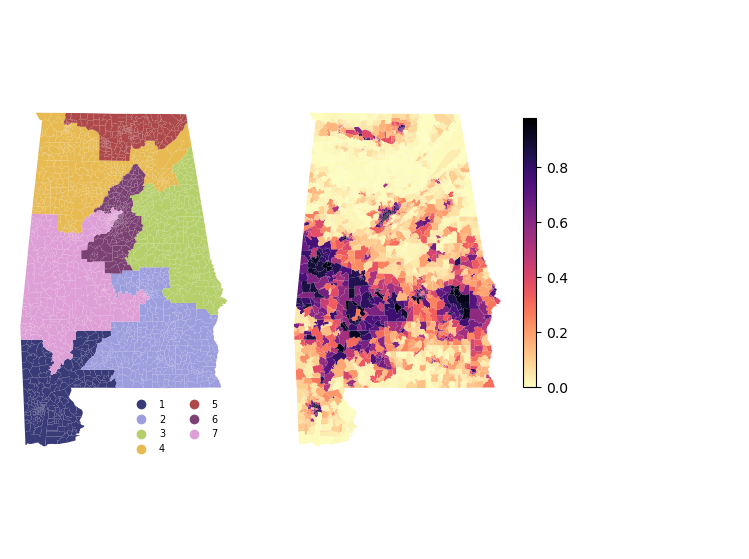
\includegraphics[trim={0cm 2cm 4cm 2},clip,scale=.75]{images/AL.png}
    \caption{\textbf{Alabama 2020 Congressional District Map, Percent Black Population by VTD} Left: The Alabama 2020 Congressional District Map under dispute. Plaintiffs argue district 7 is in violation of Section 2 of the Voting Rights Act. Right: Percentage of VTD population identifying as black, where darker colors indicate higher percentages. Note the overlap of District 7 and the blackest part of the state.}
\end{figure}

\par
Kosuke Imai of ALARM and Moon Duchin of MGGG both offered expert testimony on the matter. Each generated potential congressional maps of Alabama, and offered analysis on the ease with which a second majority-minority district could be drawn (>50\% BVAP). Duchin stated that her simulations found "literally thousands of ways" to draw two majority black districts, though she had to impliment this specification directly, such that the defendants argue it was not a "race-blind" approach. Imai also noted that that none of the generated districts had a BVAP as high as the actual district 7, though defendants argue that his "race-blind" generated plans still did not produce two majority-minority districts, only "crossover" districts. We can see that even implimenting quantitative processes such as the MCMC algorithms does not neccesarily prove gerrymandering has occured. However, it does provide courts with a means of comparing many maps, and also makes the task of creating this large number of plans much easier than if done by hand.
 
\subsection{The Areal Unit Segregation ($S^{+/-}$) Measure}\label{AUS}

In many of the cases above, including \emph{Merril v. Milligan}, a measure of BVAP is used to quantify minority populations within districts. This score is perhaps compares the minority population in a district to the districts population as a whole, and may not account for the tendency of minority populations to cluster in a state. It becomes challenging to identify \emph{segregation} that occures because of gerrymandering, or segregation that is "natural" to the minority populations distribution across a state. When it comes to quantifying segregation specifically, social scientists have been making use of areal metrics to calculate the spacial distribution of minority populations \hl{(Whitte, 1983; Reardon and O'sullivan, 2004; Echernique and Fryer Jr, 2007)}. Saporito and Maliniak (2022) build upon these measures by implimenting a nearest-neighbors algorithm to the metric, defining what they call an Areal Unit Segregation Measure ($S^{+/-}$).
\par
A ($S^{+/-}$) score contextualizes a minority population in its local geogrpahic region, relying on the idea that "the racial composition of the nearest N neighbors of any given district’s residents should be, on average, very similar to the racial composition of the district" \hl{()}. By comparing the percent of a districts residents who are black to the percent of the districts N nearest neighbors that are black, we can determine whether the district has been segregated. In this case, a positive ($S^{+/-}$) score indicates a packed district, a score of 0 is non-segregated, and a negative score indicates a cracked district. Determining the racial composition of the environment a district is situated in requires defining a "local environment". Saporito and Maliniak do so by aggregating the racial makeup of the N nearest neighbors to every resident of a potential district.
\par
We make use of Saporito and Maliniak's ($S^{+/-}$) measure in our analysis, and compare these scores bvap. It may not be clear whether one score is inherently better than another, but each provides a different persepctive on the issue of racial gerrymandering.

\section{Methods}\label{methods}
This paper utilizes both MGGG's GerryChain algorithm and the $S^{+/-}$ measure to evaluate segregation within Alabama's 2020 congressional districting map. We generate ensembles of districting plans according to Alabama's state criteria, and calculate segregation scores for each of these maps. ALARM similarly generated districting maps utilizing their SMC algorithm, which we also apply the $S^{+/-}$ measure to for comparison. In section 2.1, we discuss the legal constraints on congresssional districts. In the following sections 2.2 and 2.3, we discuss our specific methos and confirm convergence of our MCMC generated ensemble of maps. In section 3, we apply $S^{+/-}$ and BVAP measures to both our ensemble and an enseble generated with ALARM's SMC algorithm. We conclude in section 4, considering the implications of our data in section well as potential pitfalls to the methodology and areas for future research.

\subsection{Constraits on Map Generation}\label{constraints}

Alabama provides several criteria for congressional districts. These criteria state that districts must:

\begin{enumerate}
	\item be contiguous
	\item have equal populations
    \item be geographically compact
    \item preserve county and municipality boundaries as much as possible
    \item preserve communities of interest as much as possible
    \item avoid competition between incumbents
\end{enumerate}

Clearly, several of these criteria are open to interpretation, an issue that is relevant in legeslation but beyond the scope of this paper. Our algorithm is able to enforce every constraint except incumbent competition. All generated districts are continuious, and compactness is accounted for by the number of county splits; they are limited to 3 times the original number of splits. This also helps us to preserve county boundaries. As for population, districts are kept within a .5\% population deviance from the ideal, equal populations. Seeing as our plans are generated for the purpose of evaluating segregation, we do not consider opportunity districts, BVAP scores, or communities of interest. In this way, our generated maps may be considered "race-blind".

\subsection{Map Generation}\label{generation}
Using MGGG’s GerryChain library and ReCom proposal, we generated 1,000,000 districting maps of Alabama’s 7 congressional districts. We began with Alabama’s 2020 congressional district plan as a seed. We continued from the original map for 2000 iterations, and subsequently used the 2000th map as a seed for 2 more, different iterative runs. We continued in this fashion, each 2000th map being the seed for two more terative runs. It was our hope that this method, aside from inceasing the speed of computation, would create maps suitably different from eachother so that we can appropriately approximate a distribution of segregation measures.
\par
For each of the 7 districts in each of these plans, we calculated an $S^{+/-}$ score according to Saporito and Maleniak’s quantification, resulting in \hl{X} individual segregation scores. Data for these calculations comes from the 2020 US census, and includes geographies for voting tabulation districts as well as population statistics in these localities. \st{We additionally generated 35,000 segregation scores based on ALARM's 5,000 districting plans for the state for comparison.}
\subsection{Convergence Analysis}\label{convergence}

\section{Results}\label{results}

\subsection{Areal Unit Segregation Analysis}

\subsection{BVAP Comparison}

\section{Conclusion}

\end{document}